% Options for packages loaded elsewhere
\PassOptionsToPackage{unicode}{hyperref}
\PassOptionsToPackage{hyphens}{url}
\PassOptionsToPackage{dvipsnames,svgnames,x11names}{xcolor}
%
\documentclass[
  letterpaper,
  DIV=11,
  numbers=noendperiod]{scrreprt}

\usepackage{amsmath,amssymb}
\usepackage{iftex}
\ifPDFTeX
  \usepackage[T1]{fontenc}
  \usepackage[utf8]{inputenc}
  \usepackage{textcomp} % provide euro and other symbols
\else % if luatex or xetex
  \usepackage{unicode-math}
  \defaultfontfeatures{Scale=MatchLowercase}
  \defaultfontfeatures[\rmfamily]{Ligatures=TeX,Scale=1}
\fi
\usepackage{lmodern}
\ifPDFTeX\else  
    % xetex/luatex font selection
\fi
% Use upquote if available, for straight quotes in verbatim environments
\IfFileExists{upquote.sty}{\usepackage{upquote}}{}
\IfFileExists{microtype.sty}{% use microtype if available
  \usepackage[]{microtype}
  \UseMicrotypeSet[protrusion]{basicmath} % disable protrusion for tt fonts
}{}
\makeatletter
\@ifundefined{KOMAClassName}{% if non-KOMA class
  \IfFileExists{parskip.sty}{%
    \usepackage{parskip}
  }{% else
    \setlength{\parindent}{0pt}
    \setlength{\parskip}{6pt plus 2pt minus 1pt}}
}{% if KOMA class
  \KOMAoptions{parskip=half}}
\makeatother
\usepackage{xcolor}
\setlength{\emergencystretch}{3em} % prevent overfull lines
\setcounter{secnumdepth}{5}
% Make \paragraph and \subparagraph free-standing
\ifx\paragraph\undefined\else
  \let\oldparagraph\paragraph
  \renewcommand{\paragraph}[1]{\oldparagraph{#1}\mbox{}}
\fi
\ifx\subparagraph\undefined\else
  \let\oldsubparagraph\subparagraph
  \renewcommand{\subparagraph}[1]{\oldsubparagraph{#1}\mbox{}}
\fi

\usepackage{color}
\usepackage{fancyvrb}
\newcommand{\VerbBar}{|}
\newcommand{\VERB}{\Verb[commandchars=\\\{\}]}
\DefineVerbatimEnvironment{Highlighting}{Verbatim}{commandchars=\\\{\}}
% Add ',fontsize=\small' for more characters per line
\usepackage{framed}
\definecolor{shadecolor}{RGB}{241,243,245}
\newenvironment{Shaded}{\begin{snugshade}}{\end{snugshade}}
\newcommand{\AlertTok}[1]{\textcolor[rgb]{0.68,0.00,0.00}{#1}}
\newcommand{\AnnotationTok}[1]{\textcolor[rgb]{0.37,0.37,0.37}{#1}}
\newcommand{\AttributeTok}[1]{\textcolor[rgb]{0.40,0.45,0.13}{#1}}
\newcommand{\BaseNTok}[1]{\textcolor[rgb]{0.68,0.00,0.00}{#1}}
\newcommand{\BuiltInTok}[1]{\textcolor[rgb]{0.00,0.23,0.31}{#1}}
\newcommand{\CharTok}[1]{\textcolor[rgb]{0.13,0.47,0.30}{#1}}
\newcommand{\CommentTok}[1]{\textcolor[rgb]{0.37,0.37,0.37}{#1}}
\newcommand{\CommentVarTok}[1]{\textcolor[rgb]{0.37,0.37,0.37}{\textit{#1}}}
\newcommand{\ConstantTok}[1]{\textcolor[rgb]{0.56,0.35,0.01}{#1}}
\newcommand{\ControlFlowTok}[1]{\textcolor[rgb]{0.00,0.23,0.31}{#1}}
\newcommand{\DataTypeTok}[1]{\textcolor[rgb]{0.68,0.00,0.00}{#1}}
\newcommand{\DecValTok}[1]{\textcolor[rgb]{0.68,0.00,0.00}{#1}}
\newcommand{\DocumentationTok}[1]{\textcolor[rgb]{0.37,0.37,0.37}{\textit{#1}}}
\newcommand{\ErrorTok}[1]{\textcolor[rgb]{0.68,0.00,0.00}{#1}}
\newcommand{\ExtensionTok}[1]{\textcolor[rgb]{0.00,0.23,0.31}{#1}}
\newcommand{\FloatTok}[1]{\textcolor[rgb]{0.68,0.00,0.00}{#1}}
\newcommand{\FunctionTok}[1]{\textcolor[rgb]{0.28,0.35,0.67}{#1}}
\newcommand{\ImportTok}[1]{\textcolor[rgb]{0.00,0.46,0.62}{#1}}
\newcommand{\InformationTok}[1]{\textcolor[rgb]{0.37,0.37,0.37}{#1}}
\newcommand{\KeywordTok}[1]{\textcolor[rgb]{0.00,0.23,0.31}{#1}}
\newcommand{\NormalTok}[1]{\textcolor[rgb]{0.00,0.23,0.31}{#1}}
\newcommand{\OperatorTok}[1]{\textcolor[rgb]{0.37,0.37,0.37}{#1}}
\newcommand{\OtherTok}[1]{\textcolor[rgb]{0.00,0.23,0.31}{#1}}
\newcommand{\PreprocessorTok}[1]{\textcolor[rgb]{0.68,0.00,0.00}{#1}}
\newcommand{\RegionMarkerTok}[1]{\textcolor[rgb]{0.00,0.23,0.31}{#1}}
\newcommand{\SpecialCharTok}[1]{\textcolor[rgb]{0.37,0.37,0.37}{#1}}
\newcommand{\SpecialStringTok}[1]{\textcolor[rgb]{0.13,0.47,0.30}{#1}}
\newcommand{\StringTok}[1]{\textcolor[rgb]{0.13,0.47,0.30}{#1}}
\newcommand{\VariableTok}[1]{\textcolor[rgb]{0.07,0.07,0.07}{#1}}
\newcommand{\VerbatimStringTok}[1]{\textcolor[rgb]{0.13,0.47,0.30}{#1}}
\newcommand{\WarningTok}[1]{\textcolor[rgb]{0.37,0.37,0.37}{\textit{#1}}}

\providecommand{\tightlist}{%
  \setlength{\itemsep}{0pt}\setlength{\parskip}{0pt}}\usepackage{longtable,booktabs,array}
\usepackage{calc} % for calculating minipage widths
% Correct order of tables after \paragraph or \subparagraph
\usepackage{etoolbox}
\makeatletter
\patchcmd\longtable{\par}{\if@noskipsec\mbox{}\fi\par}{}{}
\makeatother
% Allow footnotes in longtable head/foot
\IfFileExists{footnotehyper.sty}{\usepackage{footnotehyper}}{\usepackage{footnote}}
\makesavenoteenv{longtable}
\usepackage{graphicx}
\makeatletter
\def\maxwidth{\ifdim\Gin@nat@width>\linewidth\linewidth\else\Gin@nat@width\fi}
\def\maxheight{\ifdim\Gin@nat@height>\textheight\textheight\else\Gin@nat@height\fi}
\makeatother
% Scale images if necessary, so that they will not overflow the page
% margins by default, and it is still possible to overwrite the defaults
% using explicit options in \includegraphics[width, height, ...]{}
\setkeys{Gin}{width=\maxwidth,height=\maxheight,keepaspectratio}
% Set default figure placement to htbp
\makeatletter
\def\fps@figure{htbp}
\makeatother
\newlength{\cslhangindent}
\setlength{\cslhangindent}{1.5em}
\newlength{\csllabelwidth}
\setlength{\csllabelwidth}{3em}
\newlength{\cslentryspacingunit} % times entry-spacing
\setlength{\cslentryspacingunit}{\parskip}
\newenvironment{CSLReferences}[2] % #1 hanging-ident, #2 entry spacing
 {% don't indent paragraphs
  \setlength{\parindent}{0pt}
  % turn on hanging indent if param 1 is 1
  \ifodd #1
  \let\oldpar\par
  \def\par{\hangindent=\cslhangindent\oldpar}
  \fi
  % set entry spacing
  \setlength{\parskip}{#2\cslentryspacingunit}
 }%
 {}
\usepackage{calc}
\newcommand{\CSLBlock}[1]{#1\hfill\break}
\newcommand{\CSLLeftMargin}[1]{\parbox[t]{\csllabelwidth}{#1}}
\newcommand{\CSLRightInline}[1]{\parbox[t]{\linewidth - \csllabelwidth}{#1}\break}
\newcommand{\CSLIndent}[1]{\hspace{\cslhangindent}#1}

\KOMAoption{captions}{tableheading}
\makeatletter
\makeatother
\makeatletter
\@ifpackageloaded{bookmark}{}{\usepackage{bookmark}}
\makeatother
\makeatletter
\@ifpackageloaded{caption}{}{\usepackage{caption}}
\AtBeginDocument{%
\ifdefined\contentsname
  \renewcommand*\contentsname{Table of contents}
\else
  \newcommand\contentsname{Table of contents}
\fi
\ifdefined\listfigurename
  \renewcommand*\listfigurename{List of Figures}
\else
  \newcommand\listfigurename{List of Figures}
\fi
\ifdefined\listtablename
  \renewcommand*\listtablename{List of Tables}
\else
  \newcommand\listtablename{List of Tables}
\fi
\ifdefined\figurename
  \renewcommand*\figurename{Figure}
\else
  \newcommand\figurename{Figure}
\fi
\ifdefined\tablename
  \renewcommand*\tablename{Table}
\else
  \newcommand\tablename{Table}
\fi
}
\@ifpackageloaded{float}{}{\usepackage{float}}
\floatstyle{ruled}
\@ifundefined{c@chapter}{\newfloat{codelisting}{h}{lop}}{\newfloat{codelisting}{h}{lop}[chapter]}
\floatname{codelisting}{Listing}
\newcommand*\listoflistings{\listof{codelisting}{List of Listings}}
\makeatother
\makeatletter
\@ifpackageloaded{caption}{}{\usepackage{caption}}
\@ifpackageloaded{subcaption}{}{\usepackage{subcaption}}
\makeatother
\makeatletter
\@ifpackageloaded{tcolorbox}{}{\usepackage[skins,breakable]{tcolorbox}}
\makeatother
\makeatletter
\@ifundefined{shadecolor}{\definecolor{shadecolor}{rgb}{.97, .97, .97}}
\makeatother
\makeatletter
\makeatother
\makeatletter
\makeatother
\ifLuaTeX
  \usepackage{selnolig}  % disable illegal ligatures
\fi
\IfFileExists{bookmark.sty}{\usepackage{bookmark}}{\usepackage{hyperref}}
\IfFileExists{xurl.sty}{\usepackage{xurl}}{} % add URL line breaks if available
\urlstyle{same} % disable monospaced font for URLs
\hypersetup{
  pdftitle={Is the Australian Benefit System fit for purpose?},
  pdfauthor={Matt Nolan},
  colorlinks=true,
  linkcolor={blue},
  filecolor={Maroon},
  citecolor={Blue},
  urlcolor={Blue},
  pdfcreator={LaTeX via pandoc}}

\title{Is the Australian Benefit System fit for purpose?}
\author{Matt Nolan}
\date{2025-01-08}

\begin{document}
\maketitle
\ifdefined\Shaded\renewenvironment{Shaded}{\begin{tcolorbox}[boxrule=0pt, breakable, sharp corners, borderline west={3pt}{0pt}{shadecolor}, enhanced, interior hidden, frame hidden]}{\end{tcolorbox}}\fi

\renewcommand*\contentsname{Table of contents}
{
\hypersetup{linkcolor=}
\setcounter{tocdepth}{2}
\tableofcontents
}
\bookmarksetup{startatroot}

\hypertarget{is-the-australian-benefit-system-fit-for-purpose}{%
\chapter*{Is the Australian Benefit System fit for
purpose?}\label{is-the-australian-benefit-system-fit-for-purpose}}
\addcontentsline{toc}{chapter}{Is the Australian Benefit System fit for
purpose?}

\markboth{Is the Australian Benefit System fit for purpose?}{Is the
Australian Benefit System fit for purpose?}

Welcome to this outline of income support for job seekers in Australia.
Please navigate to the chapters below:

\begin{itemize}
\tightlist
\item
  \protect\hyperlink{summary}{Summary}
\item
  \protect\hyperlink{introduction}{Introduction}
\item
  \protect\hyperlink{hypothetical-design}{Hypothetical Design}
\item
  \protect\hyperlink{international-comparisons}{International
  Comparisons}
\item
  \protect\hyperlink{evidence-on-policy-choices}{Evidence on Policy
  Choices}
\item
  \protect\hyperlink{references}{References}
\end{itemize}

\bookmarksetup{startatroot}

\hypertarget{summary}{%
\chapter{Summary}\label{summary}}

\bookmarksetup{startatroot}

\hypertarget{summary-1}{%
\chapter{Summary}\label{summary-1}}

This section provides a summary of the document.

\bookmarksetup{startatroot}

\hypertarget{introduction}{%
\chapter{Introduction}\label{introduction}}

\bookmarksetup{startatroot}

\hypertarget{introduction-1}{%
\chapter{Introduction}\label{introduction-1}}

The social safety net in Australia has remained unchanged in terms of
its broad principles since its inception in the 1947 Social Security Act
(cite). In broad terms the social security system intends to XXX

Two areas of reform over the past thirty years have been with regards to
an increased emphasis on work through mutual obligations and the growth
in private employment services, alongside a desire for increased system
simplicity following the two McClure reports (cite).

In order to evaluate whether a significantly different system would be
preferable, this document outlines the hypothetical design of varying
income support systems, the policy differences these systems involve,
and the international difference in these systems.

We can then use Australian and international evidence to form a view on
the trade-offs inherent in a significant reform to the Australian safety
net - and where more work is necessary.

The focus of this note is predominantly on \textbf{job loss risk},
rather than the other lifecycle risks that a social safety net supports
individuals through. However, a similar approach can be taken to also
consider these risks and the appropriate design of these payments.

\bookmarksetup{startatroot}

\hypertarget{hypothetical-design}{%
\chapter{Hypothetical Design}\label{hypothetical-design}}

\begin{Shaded}
\begin{Highlighting}[]
\FunctionTok{library}\NormalTok{(cli)}
\FunctionTok{library}\NormalTok{(tidyverse)}
\end{Highlighting}
\end{Shaded}

\begin{verbatim}
-- Attaching core tidyverse packages ------------------------ tidyverse 2.0.0 --
v dplyr     1.1.4     v readr     2.1.5
v forcats   1.0.0     v stringr   1.5.1
v ggplot2   3.5.1     v tibble    3.2.1
v lubridate 1.9.3     v tidyr     1.3.1
v purrr     1.0.2     
-- Conflicts ------------------------------------------ tidyverse_conflicts() --
x dplyr::filter() masks stats::filter()
x dplyr::lag()    masks stats::lag()
i Use the conflicted package (<http://conflicted.r-lib.org/>) to force all conflicts to become errors
\end{verbatim}

\begin{Shaded}
\begin{Highlighting}[]
\FunctionTok{library}\NormalTok{(data.table)}
\end{Highlighting}
\end{Shaded}

\begin{verbatim}

Attaching package: 'data.table'

The following objects are masked from 'package:lubridate':

    hour, isoweek, mday, minute, month, quarter, second, wday, week,
    yday, year

The following objects are masked from 'package:dplyr':

    between, first, last

The following object is masked from 'package:purrr':

    transpose
\end{verbatim}

\begin{Shaded}
\begin{Highlighting}[]
\FunctionTok{library}\NormalTok{(theme61)}
\end{Highlighting}
\end{Shaded}

\begin{verbatim}

Attaching package: 'theme61'

The following objects are masked from 'package:ggplot2':

    ggplot, ggsave, labs
\end{verbatim}

\begin{Shaded}
\begin{Highlighting}[]
\FunctionTok{library}\NormalTok{(tidyr)}
\FunctionTok{library}\NormalTok{(readxl)}
\FunctionTok{library}\NormalTok{(gghighlight)}
\FunctionTok{library}\NormalTok{(readabs)}
\end{Highlighting}
\end{Shaded}

\begin{verbatim}
Environment variable 'R_READABS_PATH' is unset. Downloaded files will be saved in a temporary directory.
You can set 'R_READABS_PATH' at any time. To set it for the rest of this session, use
    Sys.setenv(R_READABS_PATH = <path>)
\end{verbatim}

\begin{Shaded}
\begin{Highlighting}[]
\FunctionTok{library}\NormalTok{(OECD)}
\FunctionTok{library}\NormalTok{(jsonlite)}
\end{Highlighting}
\end{Shaded}

\begin{verbatim}

Attaching package: 'jsonlite'

The following object is masked from 'package:purrr':

    flatten
\end{verbatim}

\begin{Shaded}
\begin{Highlighting}[]
\FunctionTok{library}\NormalTok{(httr)}
\FunctionTok{library}\NormalTok{(Synth)}
\end{Highlighting}
\end{Shaded}

\begin{verbatim}
##
## Synth Package: Implements Synthetic Control Methods.

## See https://web.stanford.edu/~jhain/synthpage.html for additional information.
\end{verbatim}

\begin{Shaded}
\begin{Highlighting}[]
\FunctionTok{library}\NormalTok{(knitr)}
\end{Highlighting}
\end{Shaded}

\begin{center}\rule{0.5\linewidth}{0.5pt}\end{center}

\bookmarksetup{startatroot}

\hypertarget{hypothetical-design-1}{%
\chapter{Hypothetical design}\label{hypothetical-design-1}}

\hypertarget{insurance-or-a-flat-payment}{%
\section{Insurance or a flat
payment}\label{insurance-or-a-flat-payment}}

The Australian social security system was based on a similar principle
to systems implements in the United Kingdom and New Zealand at the same
time. Following the Beveridge Report's indication for the need for
\textbf{social insurance} to prevent hardship and encourage
participation following World War II, Australia introduced the Social
Security Act.

This act established a \textbf{flat rate} and \textbf{non-contributory}
payment, with the rate paid varying due to the nature of the hardship
experienced. This also took responsibility for such schemes largely away
from individual States and thereby standardised treatment across
Australia.

The element of unemployment benefits that reflects a flat rate,
non-contributory, payment is typically called \textbf{unemployment
assistance} (UA) (OECD 2024). XXX

Although this sounds similar to a \textbf{universal basic income} (UBI)
there are key distinctions:

\begin{enumerate}
\def\labelenumi{\arabic{enumi}.}
\item
  A UBI is paid to every individual, while UA is contingent on family
  structure and income.
\item
  A UBI is not directly abated at an individuals income increases - as a
  result for the same tax scale effective marginal tax rates are much
  lower for UBI recipients.
\item
  Commonly, a UBI does not involve mutual obligations or a specific
  requirement for job search while UA generally does.
\end{enumerate}

Another element of any social support system is \textbf{unemployment
insurance} (UI). The insurance element of a social support system
differs from the assistance element in terms of the payment (typically
linked to income prior to the event) and the funding mechanism
(typically involves a contribution from the individual prior to the
event which determines their eligibility).

\begin{longtable}[]{@{}
  >{\raggedright\arraybackslash}p{(\columnwidth - 6\tabcolsep) * \real{0.2784}}
  >{\raggedright\arraybackslash}p{(\columnwidth - 6\tabcolsep) * \real{0.2474}}
  >{\raggedright\arraybackslash}p{(\columnwidth - 6\tabcolsep) * \real{0.2268}}
  >{\raggedright\arraybackslash}p{(\columnwidth - 6\tabcolsep) * \real{0.2474}}@{}}
\caption{Example Table Using R}\tabularnewline
\toprule\noalign{}
\begin{minipage}[b]{\linewidth}\raggedright
Treatment
\end{minipage} & \begin{minipage}[b]{\linewidth}\raggedright
Unemployment.Assistance
\end{minipage} & \begin{minipage}[b]{\linewidth}\raggedright
Univeral.Basic.Income
\end{minipage} & \begin{minipage}[b]{\linewidth}\raggedright
Unemployment.Insurance
\end{minipage} \\
\midrule\noalign{}
\endfirsthead
\toprule\noalign{}
\begin{minipage}[b]{\linewidth}\raggedright
Treatment
\end{minipage} & \begin{minipage}[b]{\linewidth}\raggedright
Unemployment.Assistance
\end{minipage} & \begin{minipage}[b]{\linewidth}\raggedright
Univeral.Basic.Income
\end{minipage} & \begin{minipage}[b]{\linewidth}\raggedright
Unemployment.Insurance
\end{minipage} \\
\midrule\noalign{}
\endhead
\bottomrule\noalign{}
\endlastfoot
Payment relative to income & Flat Rate & Flat Rate & Relative to prio
Income \\
Employee contributions & None & None & Levy \\
Individual Means testing & Value 8 & Value 9 & Value 9 \\
Family based Means testing & Value 8 & Value 8 & Value 8 \\
Job Search obligations & Value 8 & Value 8 & Value 8 \\
Time limitations & Limited & None & Between X and X \\
\end{longtable}

\hypertarget{broad-rationale-for-distinction-in-payments}{%
\subsection{Broad rationale for distinction in
payments}\label{broad-rationale-for-distinction-in-payments}}

The reason why such policies are considered as distinct, even though
they form part of the same social safety net, is that the policy
objectives of each part of the system differ. A UA/UBI payment reflects
a \textbf{minimum income standard} related to views around poverty. A UI
system reflects an \textbf{insurance} motive where individuals can pool
ex-ante risk relating to a shock.

In terms of the \textbf{minimum income standard} this reflects in the
necessary income that is required to meet this standard. The nature of
the life event (i.e.~disability, temporary illness, redundancy, or
voluntary unemployment) and the structure of the family

In terms of \textbf{insurance} this reflects in XXX

In this note we are focused solely on \textbf{\emph{job loss risk}}.
Such an event is deemed to be \textbf{temporary} and therefore XXX

\hypertarget{the-income-unit}{%
\subsection{The income unit}\label{the-income-unit}}

The income unit reflects a set of individuals who share resources, and
so may be able to consume more than sum of their private incomes would
suggest. The primary sharing that is often considered is intra-household
sharing, or what is termed \textbf{economies of scale in the household}.

\hypertarget{the-iron-triangle}{%
\section{The Iron Triangle}\label{the-iron-triangle}}

XXX

Targeting efficiency XXX

{[}Fiscal cost{]}

{[}Poverty rates{]}

{[}Venn diagrams{]}

\hypertarget{rationale-for-varying-systems}{%
\section{Rationale for varying
systems}\label{rationale-for-varying-systems}}

Above we noted that the distinguishing policy rationale for the
unemployment assistance (UA) attribute of a support system and the
unemployment insurance (UI) attribute was a \textbf{minimum income
standard} as opposed to \textbf{lifetime income insurance}. In this
section we will be a bit more specific with this distinction.

\begin{Shaded}
\begin{Highlighting}[]
\CommentTok{\#| echo: false}

\NormalTok{data }\OtherTok{\textless{}{-}} \FunctionTok{data.frame}\NormalTok{(}
  \StringTok{\textasciigrave{}}\AttributeTok{Policy Aim}\StringTok{\textasciigrave{}} \OtherTok{=} \FunctionTok{c}\NormalTok{(}\StringTok{"Welfare{-}to{-}work"}\NormalTok{, }\StringTok{"Income Adequacy"}\NormalTok{, }\StringTok{"Fiscal Cost"}\NormalTok{,}\StringTok{"XXX"}\NormalTok{,}\StringTok{"XXX"}\NormalTok{,}\StringTok{"XXX"}\NormalTok{),}
  \StringTok{\textasciigrave{}}\AttributeTok{Unemployment Assistance}\StringTok{\textasciigrave{}} \OtherTok{=} \FunctionTok{c}\NormalTok{(}\StringTok{"Flat Rate"}\NormalTok{, }\StringTok{"None"}\NormalTok{, }\StringTok{"Value 8"}\NormalTok{, }\StringTok{"Value 8"}\NormalTok{, }\StringTok{"Value 8"}\NormalTok{,}\StringTok{"Limited"}\NormalTok{),}
  \StringTok{\textasciigrave{}}\AttributeTok{Univeral Basic Income}\StringTok{\textasciigrave{}} \OtherTok{=} \FunctionTok{c}\NormalTok{(}\StringTok{"Flat Rate"}\NormalTok{, }\StringTok{"None"}\NormalTok{, }\StringTok{"Value 9"}\NormalTok{, }\StringTok{"Value 8"}\NormalTok{, }\StringTok{"Value 8"}\NormalTok{,}\StringTok{"None"}\NormalTok{),}
  \StringTok{\textasciigrave{}}\AttributeTok{Unemployment Insurance}\StringTok{\textasciigrave{}} \OtherTok{=} \FunctionTok{c}\NormalTok{(}\StringTok{"Relative to prio Income"}\NormalTok{, }\StringTok{"Levy"}\NormalTok{, }\StringTok{"Value 9"}\NormalTok{, }\StringTok{"Value 8"}\NormalTok{, }\StringTok{"Value 8"}\NormalTok{,}\StringTok{"Between X and X"}\NormalTok{)}
\NormalTok{)}

\CommentTok{\# Generate the table}
\FunctionTok{kable}\NormalTok{(data, }\AttributeTok{caption =} \StringTok{"Example Table Using R"}\NormalTok{)}
\end{Highlighting}
\end{Shaded}

\begin{longtable}[]{@{}
  >{\raggedright\arraybackslash}p{(\columnwidth - 6\tabcolsep) * \real{0.1860}}
  >{\raggedright\arraybackslash}p{(\columnwidth - 6\tabcolsep) * \real{0.2791}}
  >{\raggedright\arraybackslash}p{(\columnwidth - 6\tabcolsep) * \real{0.2558}}
  >{\raggedright\arraybackslash}p{(\columnwidth - 6\tabcolsep) * \real{0.2791}}@{}}
\caption{Example Table Using R}\tabularnewline
\toprule\noalign{}
\begin{minipage}[b]{\linewidth}\raggedright
Policy.Aim
\end{minipage} & \begin{minipage}[b]{\linewidth}\raggedright
Unemployment.Assistance
\end{minipage} & \begin{minipage}[b]{\linewidth}\raggedright
Univeral.Basic.Income
\end{minipage} & \begin{minipage}[b]{\linewidth}\raggedright
Unemployment.Insurance
\end{minipage} \\
\midrule\noalign{}
\endfirsthead
\toprule\noalign{}
\begin{minipage}[b]{\linewidth}\raggedright
Policy.Aim
\end{minipage} & \begin{minipage}[b]{\linewidth}\raggedright
Unemployment.Assistance
\end{minipage} & \begin{minipage}[b]{\linewidth}\raggedright
Univeral.Basic.Income
\end{minipage} & \begin{minipage}[b]{\linewidth}\raggedright
Unemployment.Insurance
\end{minipage} \\
\midrule\noalign{}
\endhead
\bottomrule\noalign{}
\endlastfoot
Welfare-to-work & Flat Rate & Flat Rate & Relative to prio Income \\
Income Adequacy & None & None & Levy \\
Fiscal Cost & Value 8 & Value 9 & Value 9 \\
XXX & Value 8 & Value 8 & Value 8 \\
XXX & Value 8 & Value 8 & Value 8 \\
XXX & Limited & None & Between X and X \\
\end{longtable}

\bookmarksetup{startatroot}

\hypertarget{international-comparisons}{%
\chapter{International Comparisons}\label{international-comparisons}}

\bookmarksetup{startatroot}

\hypertarget{international-system-comparison}{%
\chapter{International system
comparison}\label{international-system-comparison}}

For comparing XX

XXX

However, a focus on only the income based social support services misses
important differences between Australia and the rest of the world.

In Australia labour market settings (employee protections, minimum and
award wages) and the roll of case managed employment services is a more
distinctive part of the safety net than across most of the OECD. {[}wage
earners welfare state{]}

{[}plot of minimum wage/average vs OECD, plot of intensity of
restrictions{]}

\hypertarget{differences-in-fiscal-expenditure-and-poverty-rates}{%
\section{Differences in fiscal expenditure and poverty
rates}\label{differences-in-fiscal-expenditure-and-poverty-rates}}

As noted above, the key advantage of the Australian social support
system is \textbf{targeting efficiency} - or that it reduces poverty at
the lowest fiscal cost.

XXX

\hypertarget{differences-in-replacement-rates}{%
\section{Differences in replacement
rates}\label{differences-in-replacement-rates}}

XXX

\hypertarget{differences-in-non-take-up-conditions}{%
\section{Differences in non-take-up
conditions}\label{differences-in-non-take-up-conditions}}

XXX

\hypertarget{differences-in-coverage}{%
\section{Differences in coverage}\label{differences-in-coverage}}

XXX

\hypertarget{differences-in-outcomes}{%
\section{Differences in outcomes}\label{differences-in-outcomes}}

\hypertarget{job-finding-and-unemployment}{%
\subsection{Job finding and
unemployment}\label{job-finding-and-unemployment}}

XX

\hypertarget{wage-scarring}{%
\subsection{Wage scarring}\label{wage-scarring}}

XX

\begin{figure}

{\centering 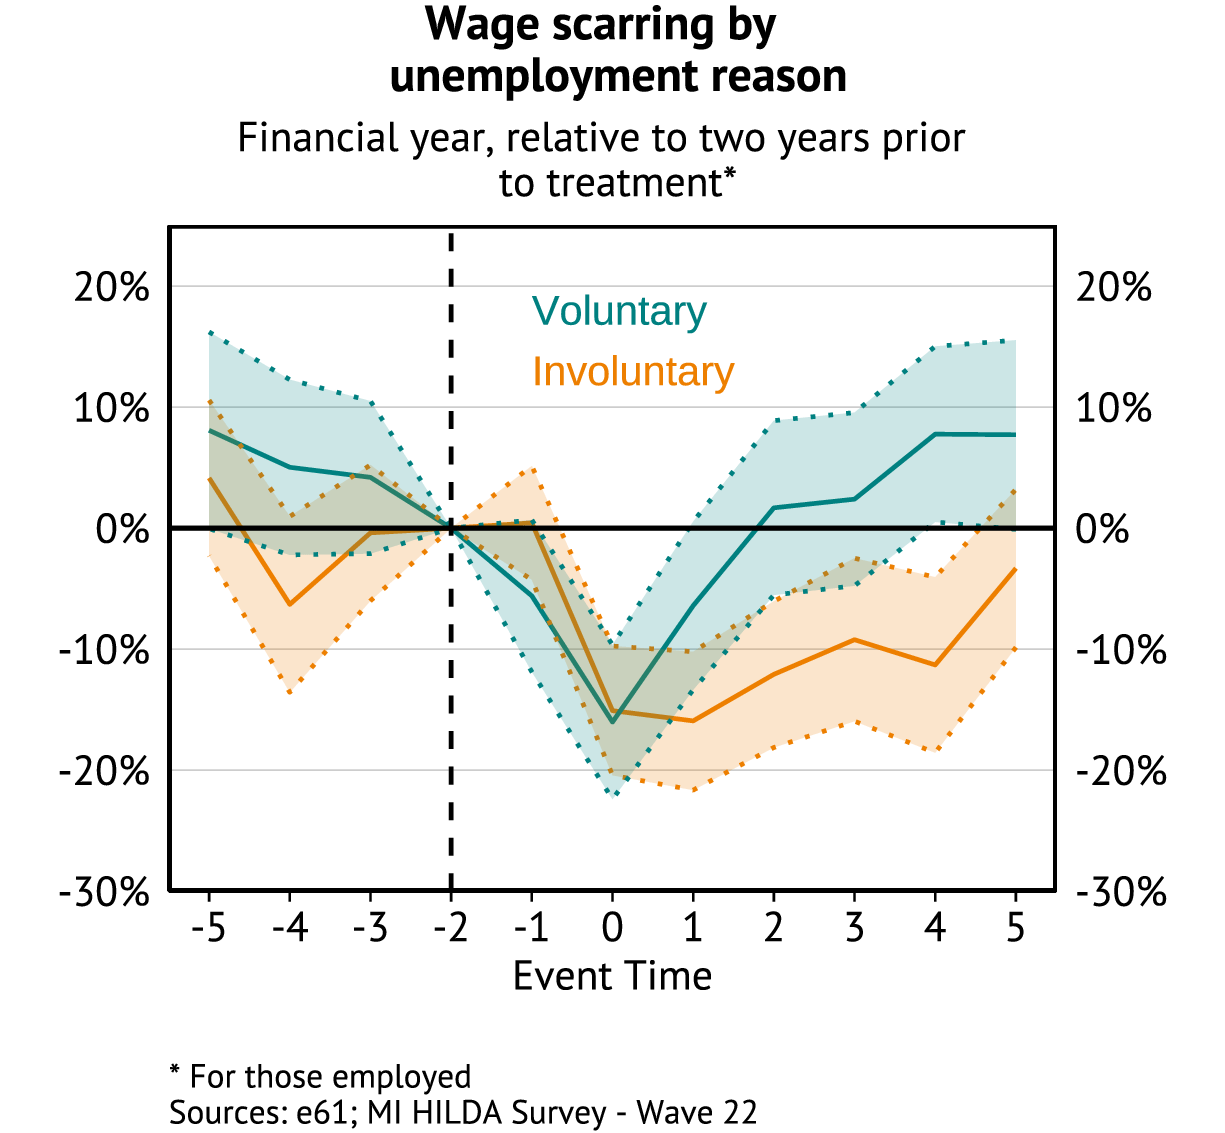
\includegraphics[width=3.125in,height=\textheight]{Inv_vol_ES.png}

}

\caption{Test}

\end{figure}

\bookmarksetup{startatroot}

\hypertarget{evidence-on-policy-choices}{%
\chapter{Evidence on Policy Choices}\label{evidence-on-policy-choices}}

\bookmarksetup{startatroot}

\hypertarget{evidence-on-system-choices}{%
\chapter{Evidence on system choices}\label{evidence-on-system-choices}}

\hypertarget{the-implications-of-mutual-obligations}{%
\section{The implications of mutual
obligations}\label{the-implications-of-mutual-obligations}}

XXX

\hypertarget{the-implications-of-the-payment-rate}{%
\section{The implications of the payment
rate}\label{the-implications-of-the-payment-rate}}

XXX

\hypertarget{the-implications-of-benefit-exhaustiontapering}{%
\section{The implications of benefit
exhaustion/tapering}\label{the-implications-of-benefit-exhaustiontapering}}

XXX

\hypertarget{the-effect-of-a-ubi}{%
\section{The effect of a UBI}\label{the-effect-of-a-ubi}}

A UBI differs from the Australian system in the following ways:

\begin{itemize}
\item
  XXX
\item
  XXX
\item
  XXX
\end{itemize}

\bookmarksetup{startatroot}

\hypertarget{references}{%
\chapter*{References}\label{references}}
\addcontentsline{toc}{chapter}{References}

\markboth{References}{References}

\hypertarget{refs}{}
\begin{CSLReferences}{1}{0}
\leavevmode\vadjust pre{\hypertarget{ref-oecd2024}{}}%
OECD. 2024. {``{Income Support, Redistribution, and Work Incentives}.''}
\url{https://www.oecd.org/en/topics/income-support-redistribution-and-work-incentives.html}.

\end{CSLReferences}



\end{document}
